% !TeX spellcheck = cs_CZ
\wikitextrule
\begin{example}\label{MAI:exam027}
  (Nalezení inverzní funkce): Funkci 
  \begin{equation*}
    y = \log_2(\sqrt{1-x^2})
  \end{equation*}
   Jsme již z různých hledisek rozebrali v příkladech \ref{fyz:fey_exam017} a \ref{MAI:exam025}. 
   Hodí se i nyní.

  {\centering
   \captionsetup{type=figure}
%  % !TeX spellcheck = cs_CZ
% K příkladu \ref{mai:exam027} \(y=\log_2{(\sqrt{1-x^2})}

\documentclass[11pt]{standalone}
\usepackage{xltxtra}
\usepackage[usenames,x11names]{xcolor}
\usepackage{tikz}
\usepackage{pgfplots}
  \pgfplotsset{compat=newest}
\usepackage{amsmath}

\begin{document}
  \begin{tikzpicture}[thick,scale=0.7, every node/.style={transform shape}]
    \begin{axis}[
      xmin = -5, xmax = 5, ymin = -5, ymax = 1.5,
   %   domain = -0.999999:0.999999,
      restrict y to domain=-30:1.5,
      unit vector ratio=1 1 1,  % axis equal
      grid = both,   % both, major
      grid style={line width=.1pt, draw=gray!20},
      major grid style={dashed, line width=.2pt, draw=gray!40},
      minor tick num=4,
      clip = true,
      clip mode=individual,
      axis x line = middle,
      axis y line = middle,
      xlabel={\(x\)},
    %  xlabel style={at=(current axis.right of origin), anchor=west},
      ylabel={\(y\)},
    %  ylabel style={at=(current axis.above origin), anchor=south},
      enlarge y limits={rel=0.13},
      enlarge x limits={rel=0.07},
    ]
    
      \addplot[color=Gold3, samples=1000, smooth, ultra thick, unbounded coords=jump, no markers, 
               domain = 0:0.9995] 
        gnuplot{log10(sqrt(1-x^2))/log10(2)};  
        
      \addplot[color=blue, samples=200, smooth, ultra thick, unbounded coords=jump, no markers, 
               domain = -5:0] 
        gnuplot{sqrt(1-2^(2*x))};  
    \end{axis}
  \end{tikzpicture}
\end{document}
   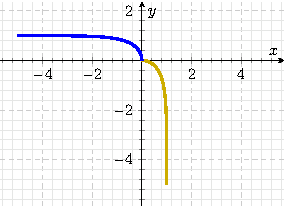
\includegraphics[width=0.5\linewidth]{mai_fig015.pdf} 
   \captionof{figure}{K příkladu \ref{MAI:exam027} \(y=\log_2{(\sqrt{1-x^2})}\) 
   \cite[s.~62]{Musilova2009MA1}
   \label{mai_fig015}}
  \par}
  
   Na obrázku \ref{mai_fig013} máme dokonce její graf, a tak vidíme, že \textbf{není} na svém 
   definičním oboru \((—1, 1)\) \textbf{prostá}. Omezme proto její definiční obor na interval 
   \( \mathcal{D} = [0, 1)\), na němž již prostá je (část grafu vpravo od osy \(y\)). Pro danou 
   hodnotu obrazu \(y \in (-\infty,0]\) můžeme již jednoznačně určit hodnotu \(x\) jednoduchou 
   úpravou:
   \begin{align*}
     y = \log_2(\sqrt{1-x^2}) &\Rightarrow \sqrt{1-x^2} = 2^y   \\
                              &\Rightarrow x^2 = 1 - 2^{2y}     \\
                              &\Rightarrow x = \sqrt{1 - 2^{2y}}
   \end{align*}
   Formální záměnou \(x \leftrightarrow y\) dostáváme inverzní funkci k funkci \(f\),
   \begin{equation*}
     y =f^{-1}(x) = \sqrt{1 - 2^{2x}}.
   \end{equation*}
   Grafy obou funkcí jsou na obrázku \ref{mai_fig015}.
\end{example}















